\documentclass[11pt,a4paper]{report}
\usepackage[utf8]{inputenc}
\usepackage[english]{babel}
\usepackage[T1]{fontenc}
\usepackage{hyperref}
\usepackage{verbatim}
\usepackage{amsmath}
\usepackage{pdfpages}
\usepackage{array}
\usepackage{amsfonts}
\usepackage{amssymb}
\usepackage{graphicx}
\usepackage{pgfplots}
\usepackage{float}
\pgfplotsset{compat=1.9}
\usepackage[left=2cm,right=2cm,top=2cm,bottom=2cm]{geometry}

\newcommand{\inlinecode}{\texttt}


\title{
\includegraphics[width=2cm]{logo-ee.png}\\
Fundamentos de Sistemas Distribuídos\\Livraria e Banco - Transações distribuídas e distribuição transparente\\MIEI}

\author{
  André Diogo\\
  
\includegraphics[width=2cm]{c.jpeg}\\
  \texttt{A75505}
  \and
  Diogo Pimenta\\
  
\includegraphics[width=2cm]{b.jpg}\\
  \texttt{A}
}

\date{\today}

\begin{document}

\maketitle

\newpage

\tableofcontents

\chapter{Introdução}

\paragraph{}Este relatório tratará de oferecer uma visão arquitetural do projeto realizado, além de considerações e justificações sobre a implementação escolhida para os diversos componentes.
\paragraph{}A descrição da API do programa estará embebida no código fonte no formato javadoc.

\chapter{Arquitetura}

\section{Visão Geral da Arquitetura}

%
%\begin{figure}[H]
%    \centering
%    \includegraphics[width=\textwidth]{kali_int_net.png}
%    \includegraphics[width=\textwidth]{kali_net.png}
%\end{figure}
\newpage

\begin{figure}[H]
  \centering
  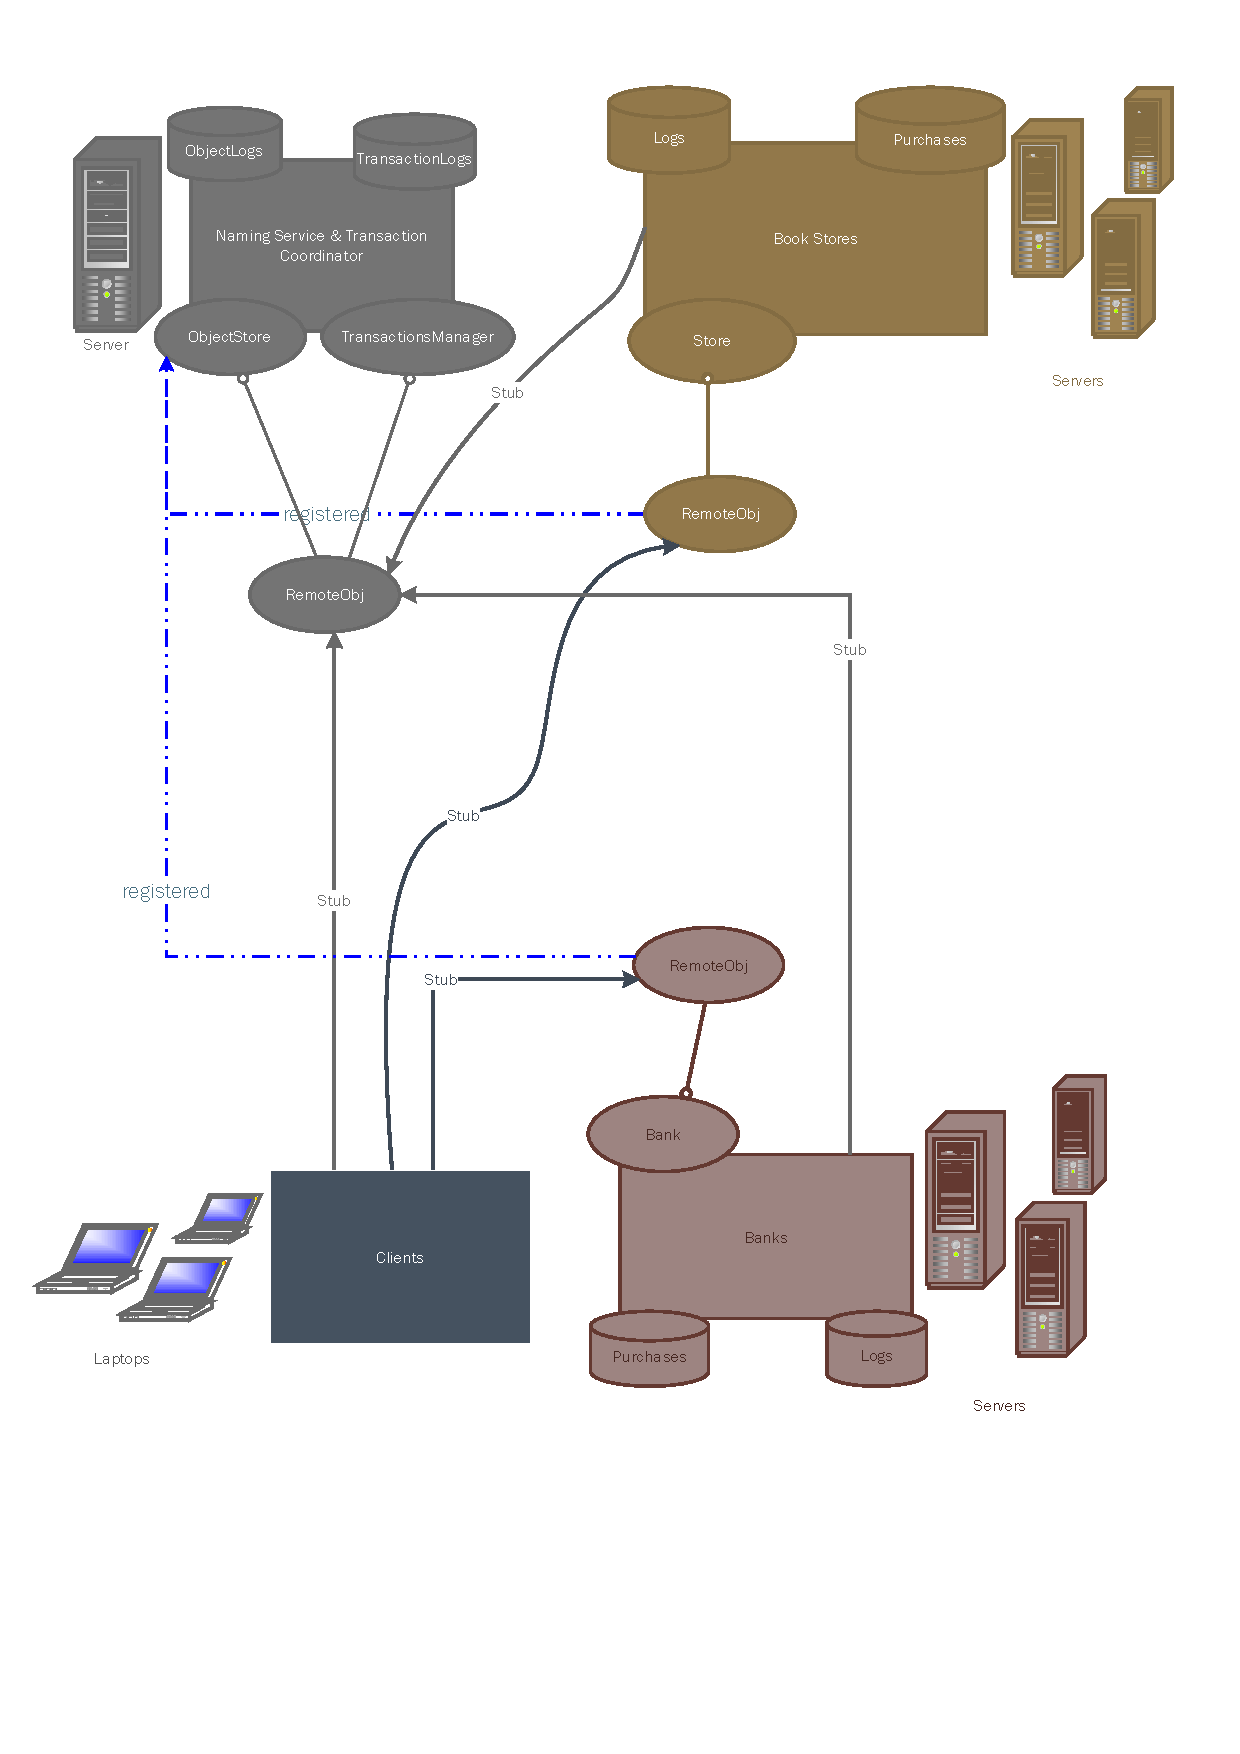
\includegraphics[scale=0.80,page=1]{Process_Architecture.pdf}
  \caption{Arquitectura dos processos.}
  \label{fig:procarq}
\end{figure}
\newpage

\paragraph{}Como mostra a figura, o nosso sistema está dependente de um processo que atua como serviço de nomes e gestor de transações conhecido por todos os outros processos.

\paragraph{}Para garantir a consistência do sistema, caso este serviço falhe, ele mantém logs que refletem o seu estado atual, para poder ser reiniciado num estado são.

\paragraph{}Temos assim ao nossa dispor a possiblidade de correr múltiplas lojas, bancos e clientes, sendo que estes se ligam apenas quando necessário recorrendo ao serviço de nomes para obterem a localização na rede do interveniente que requerem.

\section{Serviço de Nomes e Gestor de Transações}

\paragraph{}Para permitir uma configuração de rede razoavelmente dinâmica torna-se necessário ter um serviço de nomes capaz de registar servidores (quer de bancos quer de lojas) ativos, prontos para servir os clientes.

\paragraph{}Como é necessário também ter um coordenador de transações para implementar o \texitt{Two-phase commit}, o serviço de nomes tratará também de o fazer no mesmo processo.

\section{Modularidade e classes auxiliares}

\paragraph{} Para permitir uma implementação bastante modular e genérica do código envolvido na manutenção de objetos distribuídos e conexão de rede criaram-se classes auxiliares dedicadas à gestão de referências distribuídas (DistObjManager), encapsuladora de funções comuns de \texitt{leasing} de objetos e \texitt{garbage collection}, assim como importação de \texitt{Stubs
} e exportação de \textitt{Servants} (usou-se o termo Skeleton para estes na base de código); e de gestão de conexões (Server e Stub), encapsuladoras de funções comuns de gestão de ligações, registo de \texitt{handlers} e registo de \texitt{callbacks}.

\paragraph{} Estas classes abstratas tentam deferir os detalhes mais específicos (classes concretas envolvidas) para implementações mais concretas ligadas à lógica de negócio dedicada às livrarias e bancos. Tentam ser o mais \texitt{Plug 'n Play} possível, seguindo uma abordagem de inversão de controlo.

\end{document}

